\documentclass{standalone}


\usepackage{tikz}
\usepackage{xcolor}
\tikzstyle{box} = [rectangle,draw=black,thick, minimum width=2em, minimum height=2em]
\definecolor{mygray}{gray}{0.85}


\pgfdeclarelayer{L1}
\pgfsetlayers{main,L1}

\begin{document}
\begin{tikzpicture}


    \node at (0,0) (i1) {
        \begin{tikzpicture}
            \foreach \x in {0,2,4,...,30}
                {
                    \node[box, fill=cyan!20] at (\x em,0 em) {};
                }
        \end{tikzpicture}
    };


    \node at (0,-4em) (i2) {
        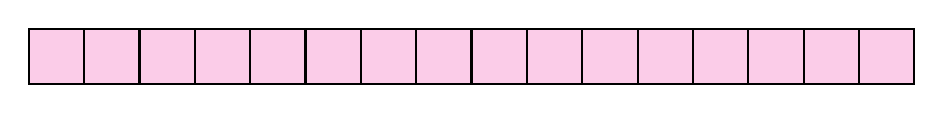
\begin{tikzpicture}
            \foreach \x in {0,2,4,...,30}
                {
                    \node[box, fill=magenta!20] at (\x em,0 em) {};
                }
        \end{tikzpicture}
    };

    \node at (0,-8em) (i3) {
        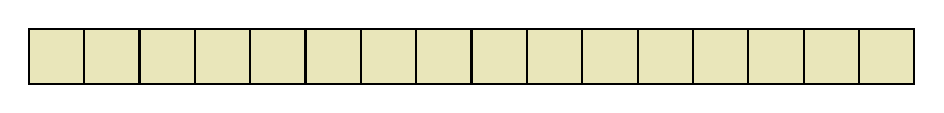
\begin{tikzpicture}
            \foreach \x in {0,2,4,...,30}
                {
                    \node[box, fill=olive!20] at (\x em,0 em) {};
                }
        \end{tikzpicture}
    };


    \draw [->,red, ultra thick] (i2.west) to [out=180,in=180] (i1.west);

    \draw [->,red, ultra thick] (i3.east) to [out=0,in=0] (i2.east);


    \draw [->,red, ultra thick] ([xshift=-3em]i3.west)  -- (i3.west)  node[pos=0, left, black] {PixelIn};

    \draw [->,red, ultra thick] (i1.east)  -- ([xshift=3em]i1.east)  node[pos=1, right, black] {PixelOut};

    \begin{pgfonlayer}{L1}
        % Compute a few helper coordinates
        \path (i1.east |- i1.north)+(-3.8,0.2) node (a) {};
        \path (i3.south -| i1.east)+(0.2,-0.8) node (b) {};
        \path[fill=green!70,rounded corners, opacity=0.3, draw=black!50, dashed]
        (a) rectangle (b);
    \end{pgfonlayer}

    \node at ([xshift=11em,yshift=-1.5em]i3.south) {\textbf{$3\times5$ Register Bank }};
\end{tikzpicture}

\end{document}